\usetikzlibrary{calc}
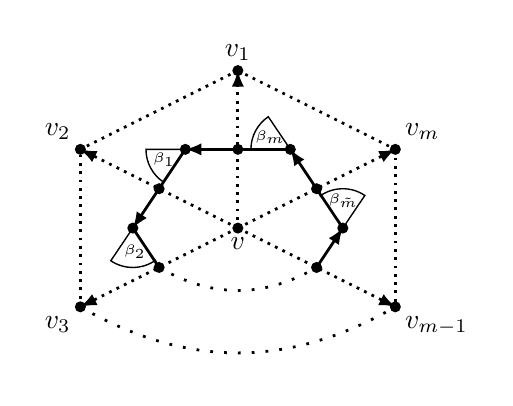
\begin{tikzpicture}[>=latex]
  % Coords
  \coordinate (V0) at (2,0);
  \coordinate (V1) at (2,2);
  \coordinate (V2) at (0,1);
  \coordinate (V3) at (4,1);
  \coordinate (V4) at (4,-1);
  \coordinate (V5) at (0,-1);
  % Arrows\tilde{\sigma}
  \draw[line width=1pt,style=dotted, ->]
    (V0) -- (V1);
  \draw[line width=1pt,style=dotted]
    (V1) --  (V2);
  \draw[line width=1pt,style=dotted, ->]
    (V0) -- (V2);
  \draw[line width=1pt,style=dotted]
    (V1) --  (V3);
  \draw[line width=1pt,style=dotted, ->]
    (V0) -- (V3);
   \draw[line width=1pt,style=dotted, ->]
    (V0) -- (V4);
  \draw[line width=1pt,style=dotted, ->]
    (V0) -- (V5);
  \draw[line width=1pt,style=dotted]
    (V5) --  (V2);
  \draw[line width=1pt,style=dotted]
    (V3) --  (V4);
  % Points
  \fill (V0) node[below] {\(v\)} circle (2pt);
  \fill (V1) node[above] {\(v_1\)} circle (2pt);
  \fill (V2) node[above left] {\(v_2\)} circle (2pt);
  \fill (V3) node[above right] {\(v_{m}\)} circle (2pt);
  \fill (V4) node[below right] {\(v_{m-1}\)} circle (2pt);
  \fill (V5) node[below left] {\(v_3\)} circle (2pt);
  \draw[line width=1pt, style=loosely dotted]
     (V5) to[bend right] (V4);
  %circumcenter
  \coordinate (CC1) at (1.333,1);
  \coordinate (CC0) at (2.666,1);
  \coordinate (CC2) at (0.666,0);
  \coordinate (CCm) at (3.333,0);
  \coordinate (CCC0) at (2,1);
  \coordinate (CCC1) at (1,0.5);
  \coordinate (CCC2) at (3,0.5);
  \coordinate (CCC3) at (1,-0.5);
  \coordinate (CCC4) at (3,-0.5);
  \fill (CC0) circle (2pt);
  \fill (CC1) circle (2pt);
  \fill (CC2) circle (2pt);
  \fill (CCm) circle (2pt);
  \fill (CCC0) circle (2pt);
  \fill (CCC1) circle (2pt);
  \fill (CCC2) circle (2pt);
  \fill (CCC3) circle (2pt);
  \fill (CCC4) circle (2pt);
  \draw[line width=1pt, ->] (CC0) -- (CC1);
  \draw[line width=1pt, ->] (CC1) -- (CC2);
  \draw[line width=1pt, ->] (CCm) -- (CC0);
  \draw[line width=1pt] (CC2) -- (CCC3);
  \draw[line width=1pt,->] (CCC4) -- (CCm);
  \draw[line width=1pt, style=loosely dotted]
     (CCC3) to[bend right] (CCC4);

%winkel
\draw[line width=0.5pt] (CC1) -- +(180:0.5) arc (180:236:0.5);
\node at ($(CC1)+(205:0.3)$) {\tiny\(\beta_1\)};
\draw[line width=0.5pt] (CC2) -- +(236:0.5) arc (236:306:0.5);
\node at ($(CC2)+(275:0.3)$) {\tiny\(\beta_2\)};
\draw[line width=0.5pt] (CC0) -- +(124:0.5) arc (124:180:0.5);
\node at ($(CC0)+(149:0.3)$) {\tiny\(\beta_m\)};
\draw[line width=0.5pt] (CCm) -- +(56:0.5) arc (56:126:0.5);
\node at ($(CCm)+(89:0.35)$) {\tiny\(\beta_{\tilde{m}}\)};
%\draw[line width=0.5pt] (V3) -- +(206.565:0.95) arc (206.565:153.435:0.95);
%\node[left] at (V3) {\(\beta_{0m}\ \)}; 
%\draw[line width=0.5pt] (V2) -- +(-26.565:0.9) arc (-26.565:26.565:0.9);
%\node[right] at (V2) {\(\ \alpha_{01}\)}; 


\useasboundingbox ([shift={(1mm,1mm)}]current bounding box.north east) rectangle ([shift={(-1mm,-1mm)}]current bounding box.south west);
\end{tikzpicture}

